\documentclass{report}
\usepackage{tikz}
\usetikzlibrary{mindmap}
\pagestyle{empty}
\begin{document}
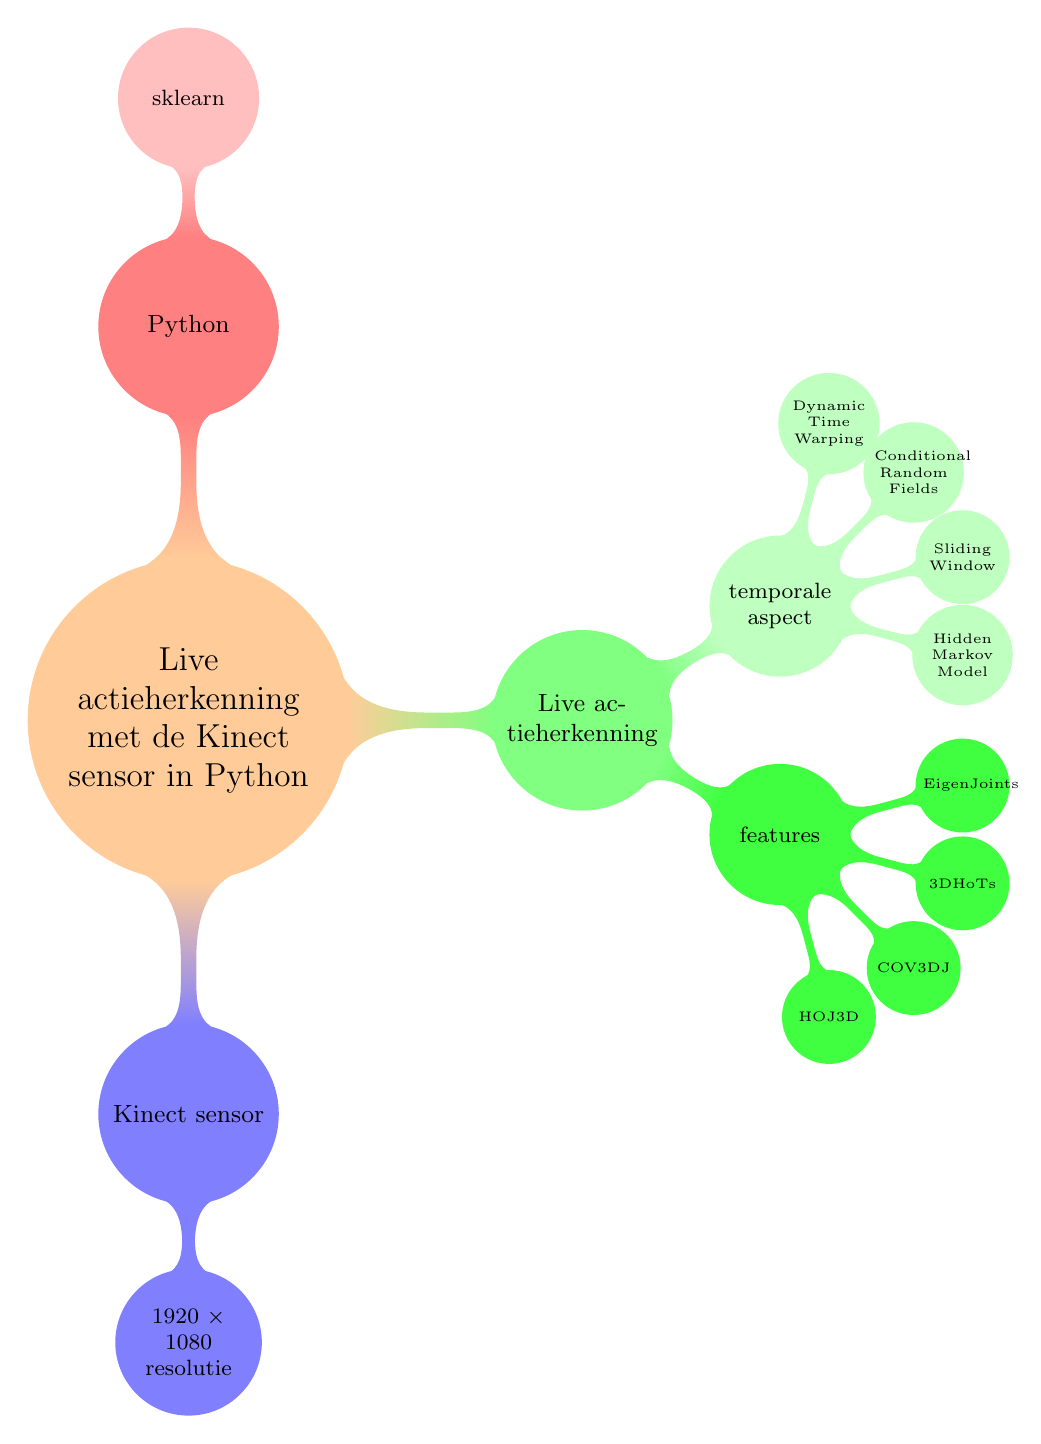
\begin{tikzpicture}[mindmap, grow cyclic, every node/.style=concept, concept color=orange!40, align= flush center,
					  level 1/.append style={level distance=5cm, sibling angle = 90}]

\node{Live actieherkenning met de Kinect sensor in Python}
	child [concept color=blue!50] { node {Kinect sensor}
		child { node {1920 $\times$ 1080 resolutie}}
	}
	child [concept color=green!50] { node {Live actieherkenning}
		child [concept color=green!75] { node {features}
			child { node {HOJ3D}}
			child { node {COV3DJ}}
			child { node {3DHoTs}}
			child { node {EigenJoints}}
		}
		child [concept color=green!25] { node {temporale aspect}
			child { node {Hidden Markov Model}}
			child { node {Sliding Window}}
			child { node {Conditional Random Fields}}
			child { node {Dynamic Time Warping}}
		}
	}
	child [concept color=red!50] { node {Python}
		child [concept color=red!25] { node {sklearn}}
	}
;

\end{tikzpicture}
\end{document}